\appendix
\backupbegin

\section{Additional}
\subsection{Speeding up Aging}

\begin{frame}[c]{Werner Syndrome}
    \large
    \begin{itemize}[<+(1)->]
        \item 'Premature aging', median age of death: 47
        \item Autosomal Recessive (does not affect carrier)
        \item Caused by mutation in WRN gene
        \item WRN important for DNA-Repair, especially after oxidative damage \cite{szekely2005werner}
    \end{itemize}

\end{frame}


\begin{frame}[c]{Artifially speed up aging}
    \large
    Study with mice injected restriction enzyme activate with drug to induce
    repeated DNA damage, they age considerably faster. Same with knocking out SIRT1 and others
\end{frame}

\section{Common Pathways}

\subsection{Effects of harsh conditions}

\begin{frame}[c]{Life Expectancy after Cancer}
    \large
    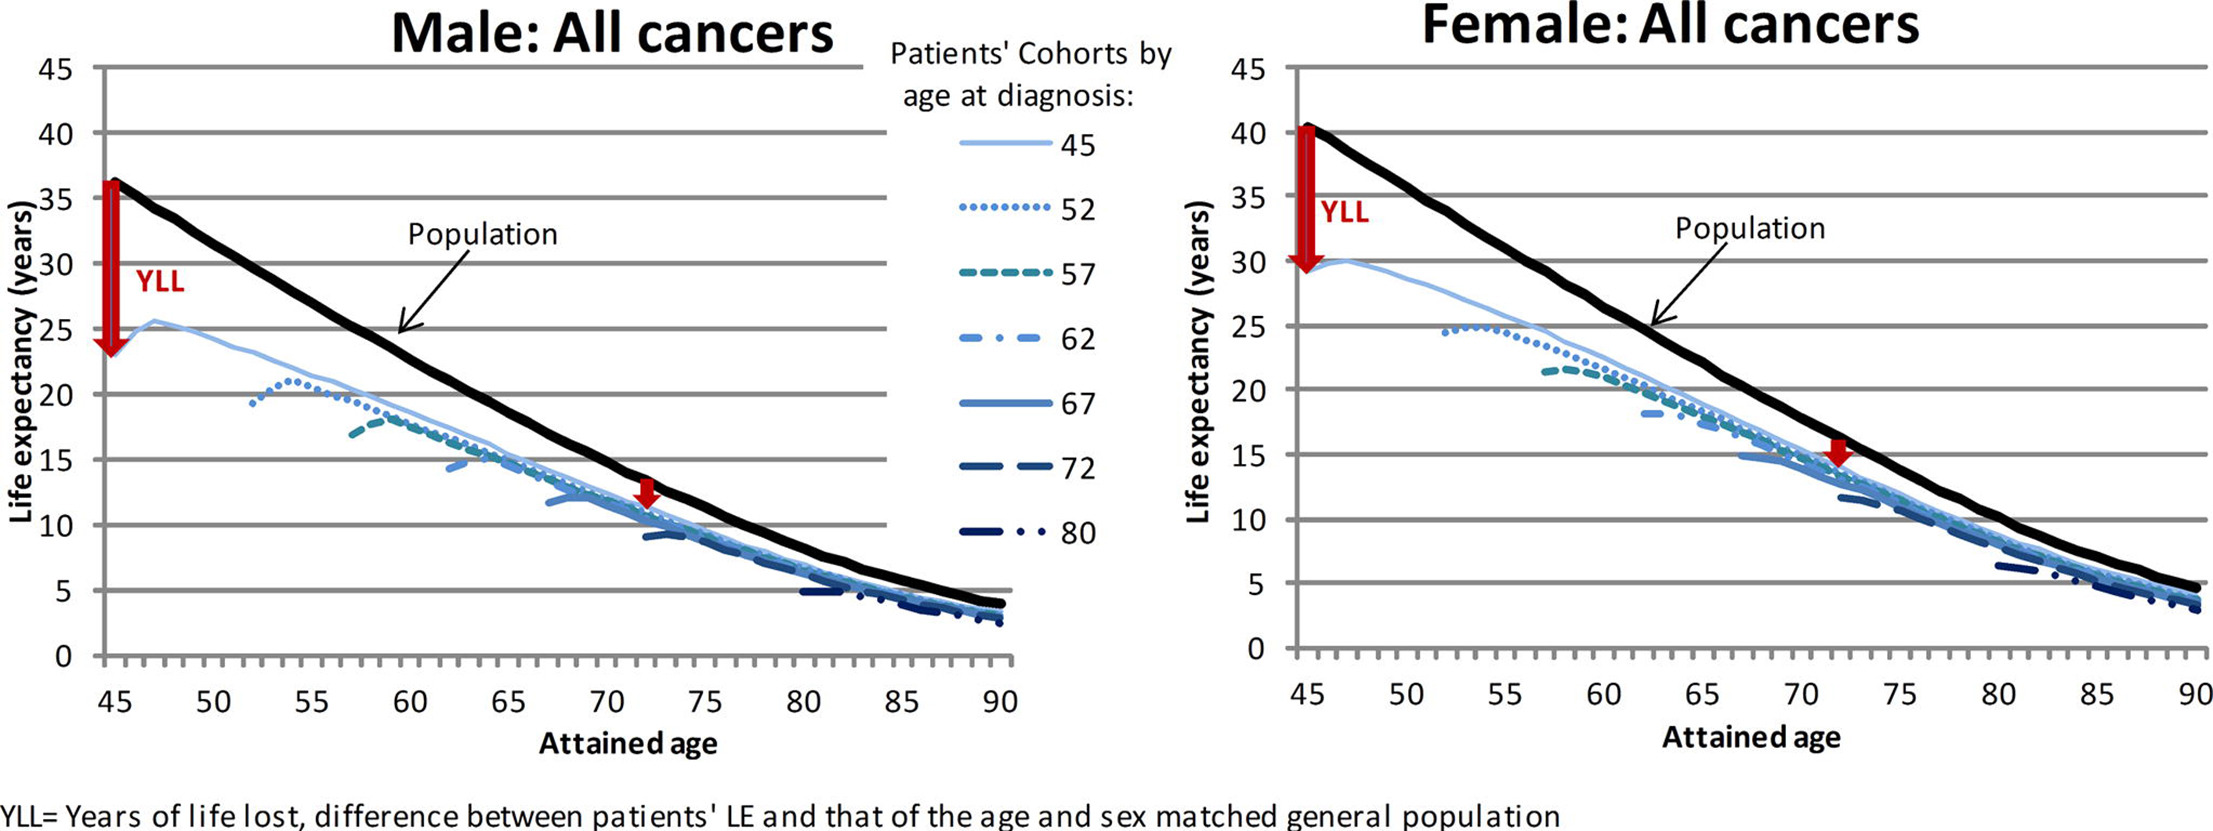
\includegraphics[width=\textwidth]{all_cancers_LE} \\
    \cite{botta2019changes}
    \newline
    \newline
    \pause
    Conclusion: Cancer causes the underlying \\ 'aging clock' to speed up \\
    reformulate to indication or something
\end{frame}

\begin{frame}[c]{Life Expectancy with Diabetes}
    \large
    Life Expectancy is at least 10 years lower with Diabetes Type 1
    \cite{livingstone2015estimated} and at least 5 years lower with Diabetes Type
    2 \cite{untitled1:online}.
    \newline
    \newline
    \pause
    Conclusion: Diabetes causes the underlying \\ 'aging clock' to speed up
\end{frame}


\begin{frame}[c]{Life Expectancy under Physiological Stress}
    \large
    \begin{aquote}{John S Wentworth \cite{Homeosta76:online}}
    There's a qualitative general pattern that various kinds of physiological
        stress - exposure to radiation or harsh chemicals (including smoking),
        chronic infection, malnutrition, sleep deprivation, etc - tend to
        accelerate aging.
    \end{aquote}
    find papers showing that these things cause hallmarks of aging to deteriorate
\end{frame}


\subsection{Diseases of Aging}

\begin{frame}[c]{Similarities of Diseases of Aging}
    \large
    \cite{CorePath13:online}
    At the cellular level:
    \begin{itemize}[<+(1)->]
        \item Decrease in cell count
        \item Increase in damaged proteins/DNA/fats
        \item Inflammation
    \end{itemize}
    \pause

    Roughly this pattern for:
    \begin{multicols}{2}
    \begin{itemize}[<+(1)->]
        \item Alzheimers
        \item Arthritis
        \item Atherosclerosis
        \item Muscle loss
        \item Osteoporosis
        \item Many more
    \end{itemize}
    \end{multicols}
\end{frame}

\begin{frame}[c]{Existence proof for common pathways}
    \large
    \begin{aquote}{John S Wentworth}
        someone who has one severe illness early is likely to have others
    \end{aquote}

    \pause
    Most severe illnesses cause the 'aging clock' to speed up. Most diseases of
    aging have similar characteristics. This is direct evidence that there are
    {\em few underlying root causes} for aging.
\end{frame}


\section{Hallmarks of Aging}

% \begin{frame}[c]{Overview of Core Mechanisms}
%     \large
%     \begin{itemize}[<+(1)->]
%         \item DNA Damage
%         \item Loss of Epigenetic Information
%         \item Mitochondria low-energy state
%         \item Telomere attrition
%         \item Unsuppressed Transposons
%     \end{itemize}
% \end{frame}


\subsection{DNA Damage}
\begin{frame}[c]{DNA Damage}
    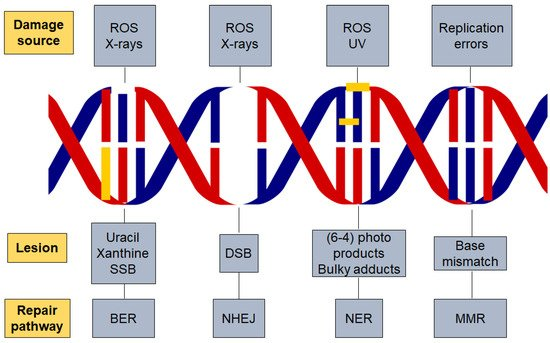
\includegraphics[width=\textwidth]{dna_damage} \\
    \cite{alhmoud2020dna}
    % turnaround a few days at most, does not accumulate - but, increase causes aging, just isn't root cause
    \pnote{Base excision repair (BER), nucleotide excision repair (NER), non-homologous end joining (NHEJ), reactive oxygen species (ROS) and DNA mismatch repair (MMR)}
\end{frame}

\subsection{Epigenetic information Loss}
\begin{frame}[c]{Epigenetic Information Loss}
    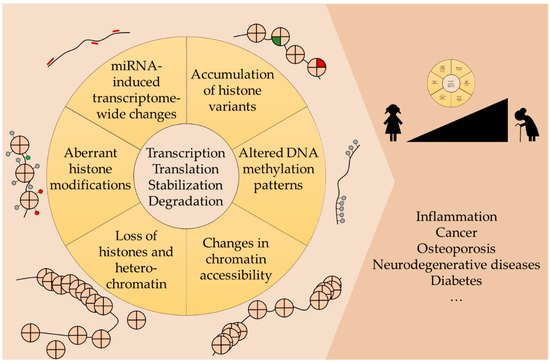
\includegraphics[width=\textwidth]{epigenetics_aging} \\
    \cite{saul2021epigenetics} \\
    % The state of an organisms epigenetics are a strong predictor for time to death \cite{lu2019dna} \\
\end{frame}

\subsection{Damaged Mitochondria}
\begin{frame}[c]{Mitochondria}
    Produce energy, explain fail-state and ROS
\end{frame}

\subsection{Telomeres}
\begin{frame}[c]{Telomeres}
    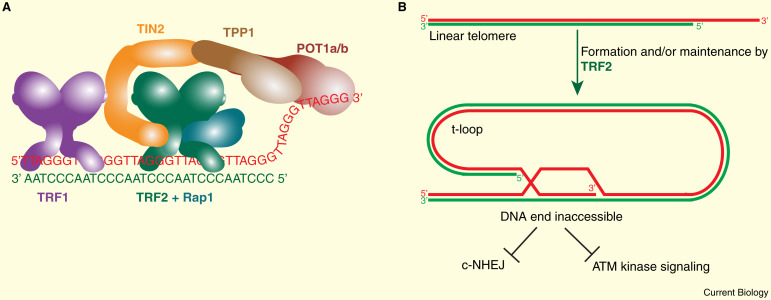
\includegraphics[width=\textwidth]{telomere_caps} \\
    \cite{schmutz2016shelterin} \\
\end{frame}

\begin{frame}[c]{Telomere attrition}
    \large
    \begin{itemize}[<+(1)->]
        \item Telomere length is only really relevant for stem cells, others don't divide
        \item Telomerase is active in stem cells
        \item True telomere damage cannot be repaired, so telomeres accumulate damage \cite{NintilTh68:online}
        \item Short telomeres cause cells to induce apoptosis
        \item So it's a good measure for total cell damage \cite{victorelli2017telomeres} 
    \end{itemize}
\end{frame}

\subsection{Transposons}
\begin{frame}[c]{Transposons}
    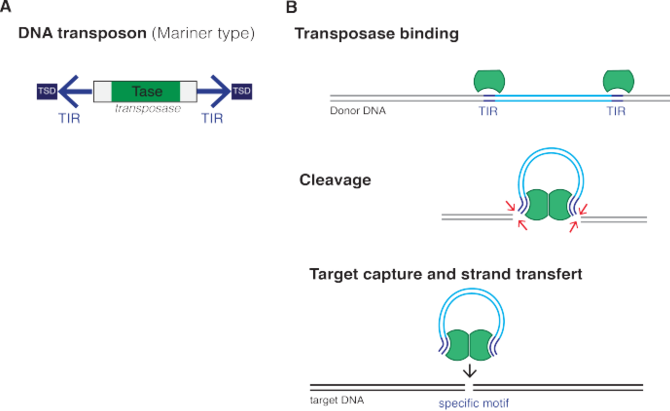
\includegraphics[height=0.8\textheight]{transposon} \\
    \pnote{
    explain transposons quick \\
    cause DNA damage, though rather additionally, as species without transposons also age \\
    about 50\% of human dna are 'dead' (broken) transposons, about 100 (of 11 major families) are still active \\
    they are suppressed most of the time, but 'let loose' a bit on other pressing matters (e.g. repairing dna damage) \\
    try to find good pictures \\
    mention that studies are being conducted currently \\
}
    \cite{walter2015transposon} \\
    Also: mice from older fathers live shorter \cite{xie2018epigenetic}
\end{frame}

\subsection{Cell Senescence}

\begin{frame}[c]{Cell Senescence}
    sending out SASP \\
    inflammation due to SASP \\
    induce apoptosis themselves or wait to get removed by immune system \\
    mice: about 8\% in young, 17\% in old \cite{folgueras2018mouse} \\
\end{frame}


\subsection{Timeframes}

\begin{frame}[c]{Timeframes for Pathways}
    \large
    \begin{itemize}[<+(1)->]
        \item DNA Damage: Repaired within Hours or faster \cite{frankenberg1989review}
        \item Senescent Cells: Removed within Days \cite{karin2018senescent}
        \item Epigenetic Markers: Varies, but most are replaced within Weeks \cite{ginno2020genome} \cite{yamagata2012rapid}
    \end{itemize}
    \pause
    Conclusion: Either the amount of Damage/Senescent Cells increases or Reparation/Removal decreases
\end{frame}

\section{Root Causes}
\subsection{Assumed Root Causes}

\begin{frame}[c]{Problem: Many Theories}
    \large
    \begin{itemize}[<+(1)->]
        \item Everything is interlinked
        \item Very hard to distinguish cause and effect
        \item At least one Theory for every Hallmark
        \item Every prestigious lab has its own Theory
        \item A lot of speculation on all sides
        \item Unclear if we can already see the full picture
        \item More research is needed
    \end{itemize}
\end{frame}

\addtocounter{framenumber}{1}
\begin{frame}[standout]
    Disclaimer: Purely Speculation including many Unknowns
\end{frame}

\begin{frame}[c]{Mitochondrial dysfunction}
    \large
    Turns out, mitochondrial dysfunction accounts for telomere-dependent senescence \cite{passos2007mitochondrial}.
\end{frame}


\begin{frame}[c]
    \large
    Assumed root causes: free radicals and transposon damage \\
    Maybe not in too much detail? Could fill 30min itself \cite{CorePath13:online} \\
    \pause

    p21 and reactive oxygen feedback for senescence \cite{passos2010feedback}
\end{frame}



\subsection{Open Questions}

\begin{frame}[c]{Questions Unanswered}
    \begin{itemize}[<+(1)->]
        \item Where are the ROS produced? Mitochondria are the top candidate - there’s a known mechanism for ROS production by mitochondria, as well as experimental evidence that mitochondrion-targeted antioxidants specifically reduce ROS-induced damage.
        \item How do the ROS and/or damaged molecules move between compartments, e.g. nucleus/cytoplasm/extracellular? I have seen very little on this, and consider it a major blindspot. I’m not sure if it’s a blindspot for the field or if I just haven’t found the right cluster of papers.
        \item Are the quantitative changes in DNA/protein/fat damage compatible with a single underlying cause? Do they match plausible estimates of ROS from dysfunctional mitochondria? Again, I haven’t seen Fermi estimates here, but I’d like to.
        \item Why is the immune system degradation related? It does degrade similarly over time, does it 'age' as well? This implies at least a second independent pathway and approach
    \end{itemize}
\end{frame}


\backupend
